\section{Model Architecture}\label{sec:model}

The whole process of CogVideoX is as follows: First, a \textbf{3D causal VAE} is used to compress the video into the latent space, and the latents are patchified and unfolded into a long sequence denoted as $z_{\text{vision}}$.
Simultaneously, we encode the textual input into text embeddings $z_{\text{text}}$ using T5~\citep{raffel2020exploring}. Subsequently, $z_{text}$ with $z_{vision}$ are concatenated along the sequence dimension. The concatenated embeddings are then fed into a stack of \textbf{expert transformer} blocks.
Finally, the model output are unpatchified to restore the original latent shape, which is then decoded using 3D causal VAE decoder to reconstruct the video. In this section, we illustrate the two main component, i.e. 3D causal VAE and expert transfomer in detail.

\subsection{3D Causal VAE} 

Compared to image data, videos encompass not only spatial information but also substantial temporal information, resulting orders of magnitude of times of data volumes and computational burden. To tackle such challenge, we propose to implement a video compression module based on 3D Variational Autoencoders (3D VAEs). Our 3D VAE incorporates three-dimentional convolutions to compress videos both spatially and temporally, achieving both higher compression ratio and largely-improved quality and continuity of video reconstruction compared to previous image VAEs.

\begin{figure}[h]
\begin{center}
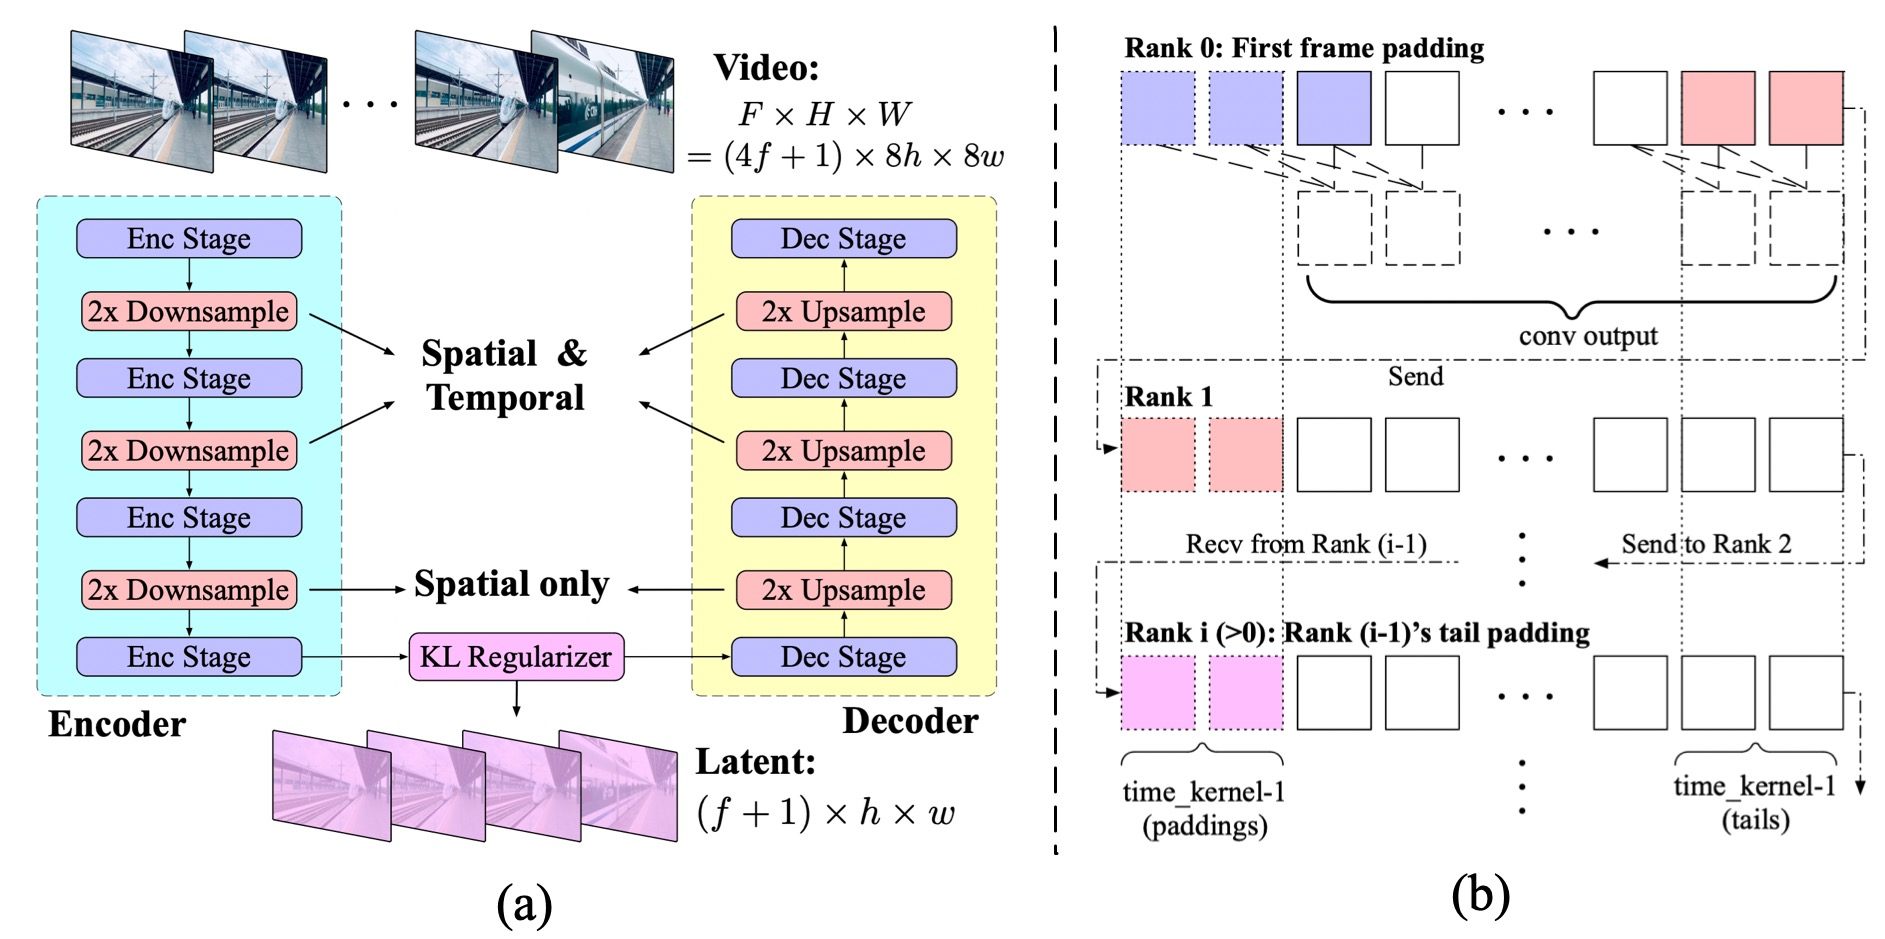
\includegraphics[width=\linewidth]{images/3dvae_combined.jpg}
\end{center}
\caption{(a) Model structure of 3D VAE. The architecture comprises an encoder, a decoder and a latent space regularizer, achieving a 4$\times$8$\times$8 compression from pixels to the latents. (b) Context parallel implementation on temporal causal convolution.}
\label{fig:3dvae_combined}
\end{figure}

The model structure of 3D VAE is shown in Figure~\ref{fig:3dvae_combined}(a). The architecture comprises an encoder, a decoder and a latent space regularizer. The encoder and decoder consist of four symmetrically arranged stages, respectively performing 2-times downsampling and upsampling by the interleaving of resnet block stacked stages. The first two rounds of downsampling and upsampling involves both the spatial and temporal dimensions, while the last round only samples spatially. This enables the 3D VAE to achieve a 4-times compression in the temporal dimension and an 8$\times$8 compression in the spatial dimensions. The Gaussian latent space is constrained by a Kullback-Leibler (KL) regularizer.

Following~\cite{yu2023language}, we implement temporally causal convolution, which places all the paddings at the beginning of the convolution space, as shown in Figure~\ref{fig:3dvae_combined}(b). This ensures the future information not to influence the present or past predictions. Given that processing videos with large number of frames introduces excessive GPU memory usage, we apply context parallel technique at the temporal dimension for 3D convolution to distribute computation among multiple devices. As illustrated by Figure~\ref{fig:3dvae_combined}(b), due to the causal nature of the convolution, each rank simply sends a segment of length $k-1$ to the next rank, where $k$ indicates the temporal kernel size. This results in relatively low communication overhead.

During actual implementation, we first train 3D VAE on lower resolutions and fewer frames to save computation. We observe that the encoding of larger resolution generalizes naturally, while extending number of frames to be encoded did not work as seamlessly. 
%yzy:先不写详细训练
Therefore, we conduct a two stage training process by first training on short videos and finetuning by context parallel on long videos. Both stages of training utilize a weighted combination of L2 loss, LPIPS~\citep{zhang2018unreasonable} perceptual loss and GAN loss from a 3D discriminator.
%Therefore we first train on videos of 17$\times$256$\times$256 with frame rate 8, by batch size of 128 and 800k training steps, and finetune by context parallel on videos of 129$\times$256$\times$256, by batch size of 16 and 200k steps. Both stages of training utilize a weighted combination of L2 loss, LPIPS~\citep{zhang2018unreasonable} perceptual loss and GAN loss from a 3D discriminator.
